\documentclass{udpreport}
\title{Cableado Estructutado}
\author{Integrantes: Francisca Carrrasco, Ignacio López.\\Profesor: José Pérez
\\Ayudante: Alexis Inzunza}
\date{Abril de 2017}
\usepackage{graphicx}
\graphicspath{ {Imagenes/} }
\udpschool{Escuela de Informática y Telecomunicaciones}

\begin{document}
\maketitle
\tableofcontents
\chapter{Actividades}
	\section{Construcción de un cable directo y un cable cruzado}
	    Para la construcción de ambos cables fueron necesarios los siguientes materiales: 
\begin{itemize}
		\item{\bf Alicate RJ45}
		\item{\bf 2 Trozos de cable de red}
		\item{\bf 4 Cabezales RJ45}
		\begin{figure}[h]
		    \centering
    	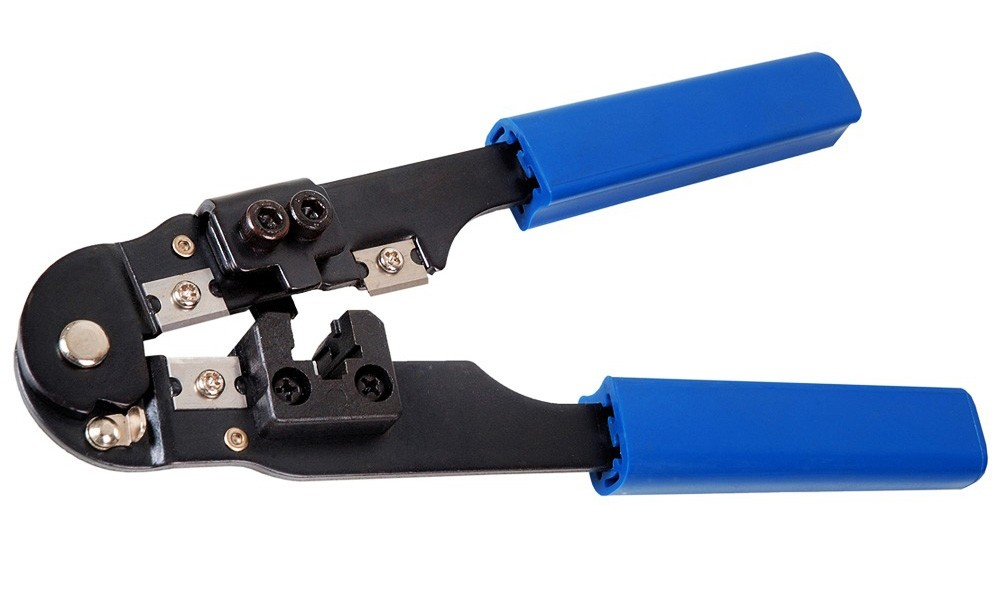
\includegraphics[width=6.5cm, height=2.5cm]{alicate.jpg}
    	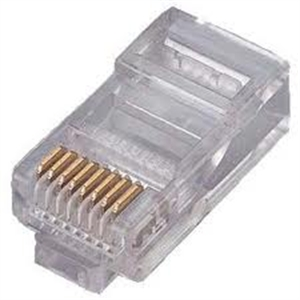
\includegraphics[width=6.5cm, height=2.5cm]{cabezal.jpeg}
    	\end{figure}
    	\\Empezando por el cable directo, lo primero que hicimos fue cortar en ambos extremos del cable una parte de su envoltura, para luego poder ordenar las trenzas según la especificación T568-A o T568-B, ambas sirven (nosotros elegimos la T568-A). Una vez ordenados lo siguiente por hacer fue cortar la punta de los pares para que así, al estar del mismo largo pudieran entrar dentro del cabezal RJ45 (hay que verificar que todos los hilos lleguen hasta el fondo), finalmente insertamos el cabezal en el alicate RJ45 (o crimpeador) teniendo cuidado de que no se mueva ningún hilo y lo apretamos para que así quede firme.
    	\\Una vez hecho esto seguimos los mismos pasos para el otro extremo del cable y debemos usar la misma especificación que elegimos anteriormente (de esto depende si el cable que acabamos de construir es un cable directo o cruzado).
    	\\Para hacer un cable cruzado las instrucciones son exactamente las mismas, con la única diferencia de que los pares de ambos extremos deben estar siguiendo distintas especificaciones, es decir, un extremo debe seguir la especificación T568-A y el otro la T568-B.
    	\begin{figure}[h]
		    \centering
    	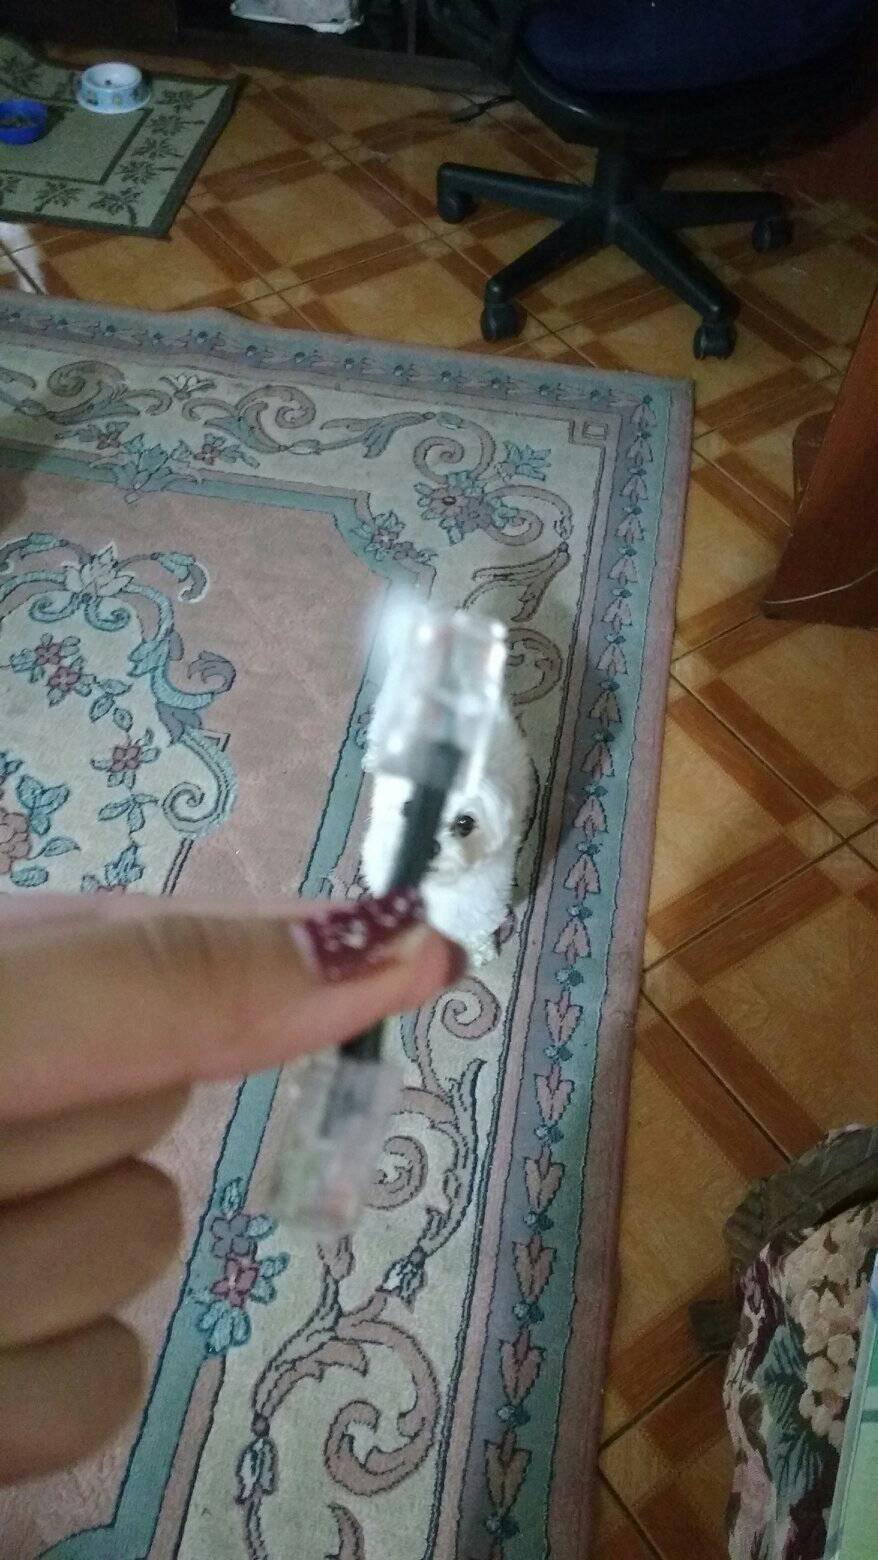
\includegraphics[width=4cm, height=4.5cm]{cable.jpg}
    	\end{figure}
\end{itemize}
	\section{Cuestionario e Investigación}
		\begin{itemize}
		\item{\bf 1.- Describa brevemente las categorías existentes de cable UTP y sus usos.} 
\\Existen las siguientes categorías:
Categoría 1: usado en líneas telefónicas y módem de banda ancha 
Categoría 2: utilizado  en algunas redes antiguas Apple-Talk (conjunto de protocolos desarrollados por Apple Inc. para la interconexión de redes locales)
Categoría 3: usado como cable horizontal y como vertical. Entre las principales aplicaciones son:  Ethernet10Base-T y Token Ring(una arquitectura de red con topología física en anillo y usando un frame llamado token que viaja alrededor del anillo).
Categoría 4: usado en redes Token Ring, 10Base-T, 10Base-T4, el cual ha decaído por desuso.
Categoría 5: utilizados en redes como Fast Ethernet, serviciosbasicos de telefonía, Token Ring, ATM(modo de transferencia asíncrona),se utiliza para ejecutar CDDI( especificaciones para permitir) el establecimiento de comunicaciones en red de área local a 100 Mbps sobre hilo de cobre)
Categoría 5e: fue creada expresamente como una mejora de la categoría 5 para poder soportar Gigabit Ethernet (1000BASE-T) 
Categoría 6: es compatible con redes 10BASE-T, 100BASE-TX y 1000BASE-TX (Gigabit Ethernet). Son muchas las empresas que realizan la instalación de categoría 6 para soportar Gigabit Ethernet en lugar de utilizar la categoría 5e.
Categoría 6a: al contrario que la categoría 6, sí que tiene una aplicación exclusiva para ella: 10GBASE-T, 
Categoría 7:  fue creado para permitir 10 Gigabit Ethernet sobre 100 metros de cableado de cobre.El inconveniente de esta categoría es el tipo de conector seleccionado que es un RJ-45 de 1 pines. 
Categoría 7a: fue creado para permitir 10 Gigabit con ethernet sobre 100 metros de cableado de cobre y para nuevas aplicaciones por venir.  Es un estándar de cable para ethernet y otras tecnologías de interconexión que puede hacerse compatible con los tradicionales cables de ethernet de categoría 5, categoría 6, categoría 6A y de categoría 7
Categoría 8: norma en desarrollo. Aun sin aplicaciones
Categoría 9 y Categoría 10: norma en creación
        \item{\bf 2.- ¿Para qué situaciones debería utilizar STP? Explique.}
 \\Este tipo de cable, de alta velocidad y tendido interior, solo se utiliza en áreas de intenso ruido eléctrico, ya que está diseñada para reducir la absorción del ruido eléctrico
\end{itemize}
\chapter{Conclusión}
    Con la realización de este laboratorio e informe entendimos la importancia de saber cuales son lo usos que posee cada tipo de cable y lo relevante que es tener en cuenta la categoría del mismo, puesto que con estos conocimientos se puede tomar la mejor decisión a la hora de tener diseñar un cableado estructurado como por ejemplo para implementar una LAN, tambíen pudimos conocer los estándares que se utilizan en el cableado estructurado, incluyendo sus utilidades y funciones.
\begin{thebibliography}{x}

\bibitem{mac} \textsc{Mac Vendors},
\textit{http://www.macvendors.com/}

\bibitem{hp} \textsc{HP},
\textit{http://www8.hp.com/cl/es/products/desktops/product-detail.html?oid=7485168}

\bibitem{cisco} \textsc{Cisco},
\textit{http://www.cisco.com/c/en/us/support/switches/catalyst-2960-24tt-l-switch/model.html}

\bibitem{blueline} \textsc{Blue Line},
\textit{http://www.blue-line.es/index.php/cobre/cat5-utp/9-cat5eutpcable.html}

\end{thebibliography}
\end{document}
Contact GitHub 
